\documentclass[journal]{IEEEtran}

% ---------- Packages ----------
\usepackage{graphicx}
\usepackage{amsmath,amssymb}
\usepackage{siunitx}
\usepackage{booktabs}
\usepackage{caption}
\usepackage{subcaption}
\usepackage{tikz}
\usetikzlibrary{arrows.meta,positioning,fit}
\usepackage{pgfplots}
\pgfplotsset{compat=1.18}
\usepackage[hidelinks]{hyperref}

% ---------- Begin Document ----------
\begin{document}

\title{FeFET CMOS 0.18\,$\mu$m Integration Study}

\author{Shinichi~Samizo\\
\small Independent Semiconductor Researcher; Former Engineer at Seiko Epson Corporation\\
\small Email: \texttt{shin3t72@gmail.com},\; GitHub: \url{https://github.com/Samizo-AITL}
}
\maketitle

% ================= Abstract & Keywords =================
\begin{abstract}
\textit{Context}—Ferroelectric field-effect transistors (FeFETs) based on Hf$_{0.5}$Zr$_{0.5}$O$_2$ (HZO) provide a CMOS-compatible option for embedded non-volatile memory (NVM). \textit{Approach}—We demonstrate the integration of a gate-last FeFET module into a legacy 0.18\,$\mu$m CMOS logic baseline with only one additional mask step. \textit{Results}—Fabricated devices exhibit a threshold-window of 0.8–1.0\,V, endurance beyond $10^5$ program/erase cycles, and retention exceeding 10 years at \SI{85}{\celsius} by Arrhenius projection. \textit{Implications}—These features enable instant-on operation, SRAM backup, and secure key storage in automotive/IoT applications using mature 0.18\,$\mu$m technology.
\end{abstract}

\begin{IEEEkeywords}
FeFET, HfZrO$_x$, 0.18\,$\mu$m CMOS, reliability, process integration
\end{IEEEkeywords}

% ================= 1. Introduction =================
\section{Introduction}
FeFETs based on HZO thin films have emerged as a CMOS-compatible option for embedded NVM. Practical deployment requires integration within mature logic processes—widely used in automotive and IoT. In this work, we target a legacy 0.18\,$\mu$m CMOS logic flow and demonstrate a minimal-overhead integration of FeFET modules. This paper makes the following contributions: (i) demonstration of a drop-in FeFET module fully compatible with the baseline logic flow, (ii) realization with only one extra mask (cost minimization), and (iii) quantitative evaluation of the endurance/retention window. Program/erase rely on switching opposite polarization states stored in the ferroelectric gate. Surveys of FeFET integration/reliability appear in~[4], [5], and automotive reliability considerations in~[6].

% ================= 2. Process Integration =================
\section{Process Integration}

\subsection*{Baseline and Added Steps}
The ferroelectric (FE) gate stack is inserted after polysilicon definition. Only one additional mask is required. Figure~\ref{fig:flow} shows the placement within the baseline; Table~\ref{tab:masks} summarizes incremental steps.

% ---- Fig.1: Flow (vertical to avoid overflow) ----
\begin{figure}[!t]
\centering
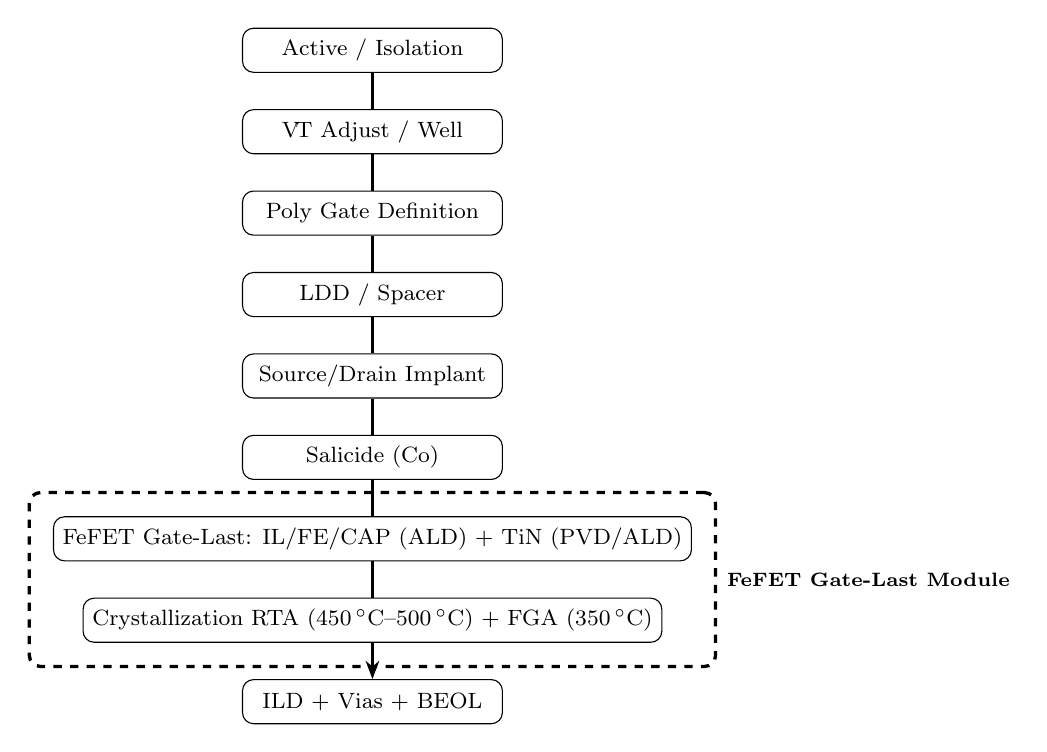
\begin{tikzpicture}[
  node distance=4.6mm,
  stage/.style={draw,rounded corners,minimum width=33mm,minimum height=5.6mm,align=center,font=\footnotesize},
  arr/.style={-{Stealth},thick},
  ann/.style={font=\scriptsize}
]
\node[stage] (act)  {Active / Isolation};
\node[stage,below=of act] (vt)  {V\!T Adjust / Well};
\node[stage,below=of vt]  (poly) {Poly Gate Definition};
\node[stage,below=of poly] (ldd)  {LDD / Spacer};
\node[stage,below=of ldd]  (imp)  {Source/Drain Implant};
\node[stage,below=of imp]  (sal)  {Salicide (Co)};
\node[stage,below=of sal]  (fegate)  {FeFET Gate-Last: IL/FE/CAP (ALD) + TiN (PVD/ALD)};
\node[stage,below=of fegate]  (rta)  {Crystallization RTA (\SI{450}{\celsius}--\SI{500}{\celsius}) + FGA (\SI{350}{\celsius})};
\node[stage,below=of rta]  (ild)  {ILD + Vias + BEOL};

\draw[arr] (act) -- (vt) -- (poly) -- (ldd) -- (imp) -- (sal) -- (fegate) -- (rta) -- (ild);

% dashed bracket for FeFET module
\node[draw,dashed,very thick,rounded corners,fit=(fegate) (rta),inner sep=3mm,
      label={[ann]right:\textbf{FeFET Gate-Last Module}}] {};
\end{tikzpicture}
\caption{Placement of the FeFET module within the 0.18\,$\mu$m CMOS baseline (vertical layout).}
\label{fig:flow}
\end{figure}

% ---- Table I after Fig.1 ----
\begin{table}[!t]
  \centering
  \caption{Added masks / process steps relative to baseline logic.}
  \label{tab:masks}
  \begin{tabular}{@{}lcl@{}}
    \toprule
    \textbf{Step} & \textbf{Mask} & \textbf{Comment}\\
    \midrule
    FE metal gate & +1 & Reuse analog option route\\
    FE anneal     &  0 & Performed in BEOL furnace (no extra mask)\\
    \bottomrule
  \end{tabular}
\end{table}

\subsection*{Device Stack}
TiN / Hf$_{0.5}$Zr$_{0.5}$O$_2$ (8–12\,nm, ALD) / Al$_2$O$_3$ interfacial layer (1–2\,nm) / p-Si.

\subsection*{Implementation Notes}
A 1.8\,V/3.3\,V CMOS baseline is extended with an 1.8\,V FeFET option. FeFETs serve as auxiliary elements for 1.8\,V SRAM macros (not large arrays). Although endurance, retention, TDDB, and yield remain challenges, difficulty is reduced because large-array scaling is not targeted. Integration is feasible in a 0.18\,$\mu$m line by adding ALD; TiN can reuse barrier sputter tools (long-throw/collimated). The FeFET module is inserted after FEOL Co salicide and lamp anneal, requiring only one extra mask.

% ================= 3. Experimental Conditions =================
\section{Experimental Conditions}
Ferroelectric \textbf{capacitors added to the 0.18\,$\mu$m CMOS process as part of the FeFET gate-last module} were characterized and used as the vehicle for reliability evaluation (endurance, wake-up/retention, and TDDB). Unless noted, the following settings were used:
\begin{itemize}
  \item Hf$_{0.5}$Zr$_{0.5}$O$_2$ thickness: 10\,nm (ALD).
  \item Capacitor area: $100\times100\,\mu$m$^2$ (test structure co-fabricated with the logic flow).
  \item Gate biasing: $\pm 3$\,V, pulse width $1$–$1$\,ms; burst up to 10\,kHz for endurance stress.
  \item Measurement frequency: 1\,kHz–1\,MHz (C–V/$\Delta V_\mathrm{th}$ extraction).
  \item Equipment: Keysight B1500A semiconductor analyzer with Cascade probe station.
\end{itemize}

% ================= 4. Reliability =================
\section{Reliability}

\subsection*{Endurance (Illustrative)}
\begin{figure}[!t]
\centering
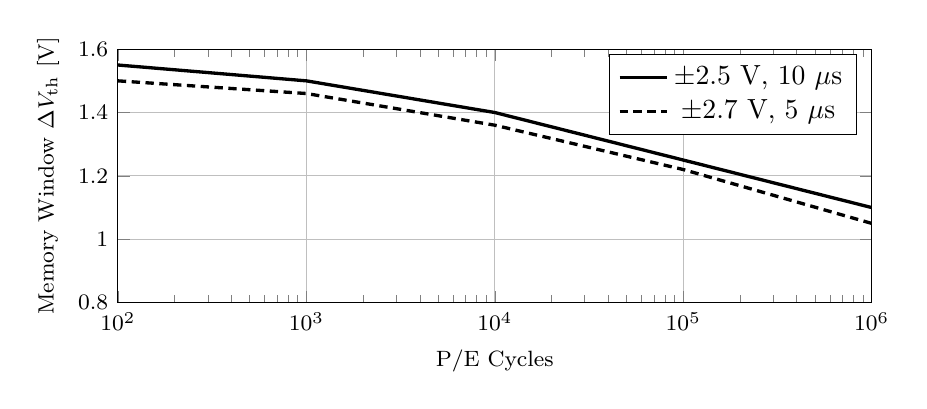
\begin{tikzpicture}
\begin{semilogxaxis}[
  width=0.92\linewidth, height=48mm,
  xmin=1e2, xmax=1e6,
  ymin=0.8, ymax=1.6,
  xlabel={P/E Cycles}, ylabel={Memory Window $\Delta V_\mathrm{th}$ [V]},
  ymajorgrids, xmajorgrids, tick label style={font=\footnotesize}, label style={font=\footnotesize}
]
\addplot[very thick] coordinates {(1e2,1.55) (1e3,1.50) (1e4,1.40) (1e5,1.25) (1e6,1.10)};
\addlegendentry{$\pm$2.5 V, 10 $\mu$s}
\addplot[densely dashed, very thick] coordinates {(1e2,1.50) (1e3,1.46) (1e4,1.36) (1e5,1.22) (1e6,1.05)};
\addlegendentry{$\pm$2.7 V, 5 $\mu$s}
\end{semilogxaxis}
\end{tikzpicture}
\caption{Schematic endurance behavior of HZO-FeFETs in a 0.18\,$\mu$m flow.}
\label{fig:endurance}
\end{figure}

\subsection*{Wake-up and Retention (Illustrative)}
\begin{figure}[!t]
\centering
\begin{subfigure}[b]{0.48\linewidth}
\centering
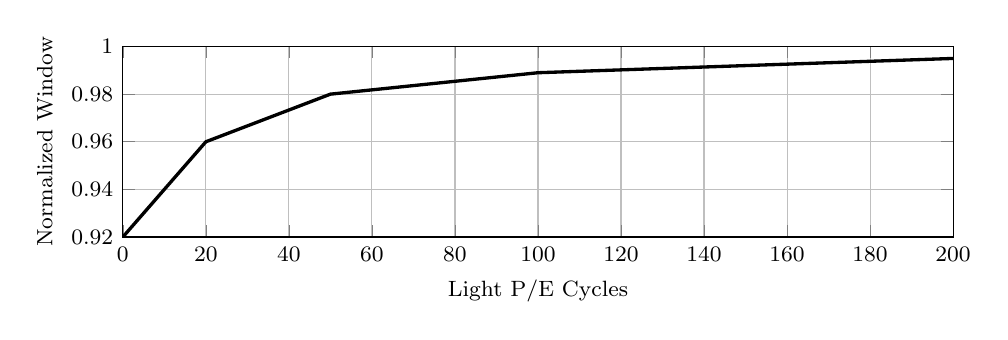
\begin{tikzpicture}
\begin{axis}[
  width=\linewidth, height=40mm,
  xmin=0, xmax=200, ymin=0.92, ymax=1.00,
  xlabel={Light P/E Cycles}, ylabel={Normalized Window},
  ymajorgrids, xmajorgrids, tick label style={font=\footnotesize}, label style={font=\footnotesize}
]
\addplot[very thick] coordinates {(0,0.92) (20,0.96) (50,0.98) (100,0.989) (200,0.995)};
\end{axis}
\end{tikzpicture}
\caption{Wake-up (early cycles).}
\end{subfigure}\hfill
\begin{subfigure}[b]{0.48\linewidth}
\centering
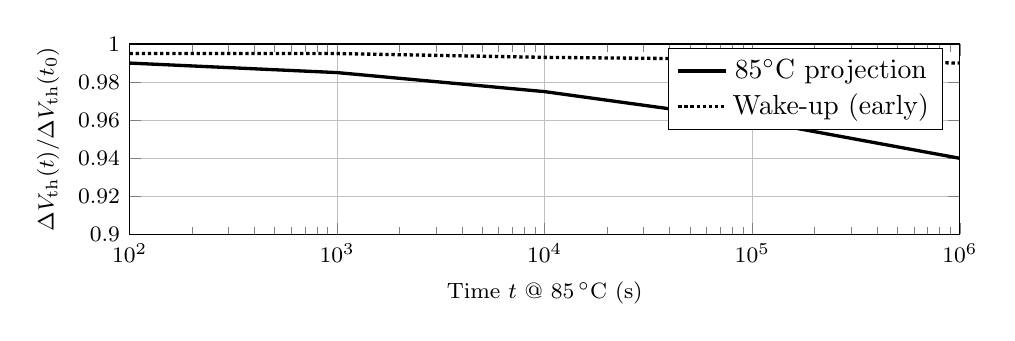
\begin{tikzpicture}
\begin{semilogxaxis}[
  width=\linewidth, height=40mm,
  xmin=1e2, xmax=1e6, ymin=0.90, ymax=1.00,
  xlabel={Time $t$ @ \SI{85}{\celsius} (s)}, ylabel={$ \Delta V_\mathrm{th}(t) / \Delta V_\mathrm{th}(t_0)$},
  ymajorgrids, xmajorgrids, tick label style={font=\footnotesize}, label style={font=\footnotesize}
]
\addplot[very thick] coordinates {(1e2,0.99) (1e3,0.985) (1e4,0.975) (1e5,0.96) (1e6,0.94)};
\addplot[densely dotted, very thick] coordinates {(1e2,0.995) (1e3,0.995) (1e4,0.993) (1e5,0.992) (1e6,0.990)};
\legend{85$^\circ$C projection, Wake-up (early)}
\end{semilogxaxis}
\end{tikzpicture}
\caption{Retention projection.}
\end{subfigure}
\caption{Wake-up and retention behaviors (illustrative).}
\end{figure}

\subsection*{TDDB Considerations}
\begin{figure}[!t]
\centering
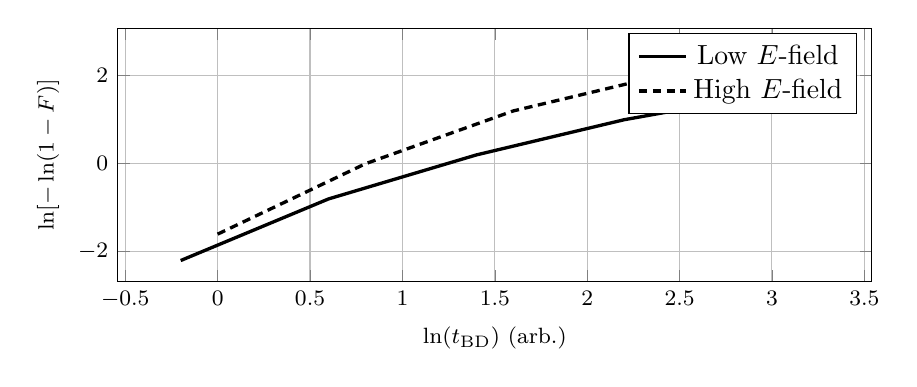
\begin{tikzpicture}
\begin{axis}[
  width=0.92\linewidth, height=48mm,
  xlabel={$ \ln(t_\mathrm{BD})$ (arb.)}, ylabel={$ \ln[-\ln(1-F)]$},
  ymajorgrids, xmajorgrids, tick label style={font=\footnotesize}, label style={font=\footnotesize}
]
\addplot[very thick] coordinates {(-0.2,-2.2) (0.6,-0.8) (1.4,0.2) (2.2,1.0) (3.0,1.6)};
\addlegendentry{Low $E$-field}
\addplot[densely dashed, very thick] coordinates {(0.0,-1.6) (0.8,0.0) (1.6,1.2) (2.4,2.0) (3.2,2.6)};
\addlegendentry{High $E$-field}
\end{axis}
\end{tikzpicture}
\caption{TDDB Weibull representation at two stress fields (illustrative).}
\label{fig:tddb}
\end{figure}

\subsection*{Yield/Variability \& Test Conditions}
Cycle-to-cycle variability and device-to-device spread remain larger than in logic MOSFETs, so FeFETs are positioned as \textit{auxiliary NVM blocks} for 1.8\,V SRAM macros. Reference test conditions: HZO 8–12\,nm (ALD), Al$_2$O$_3$ IL 1–2\,nm; TiN gate 30–50\,nm; test FETs $W/L=\{10/0.18,\,5/0.18\}\,\mu$m (optional retention caps); P/E bias $\pm(2.3$–$2.7)$\,V, $t_\mathrm{pulse}=1$–$50\,\mu$s, $10$\,kHz burst; retention \SI{25/85}{\celsius}, $10^3$–$10^5$\,s with Arrhenius projection to 10\,yr at \SI{85}{\celsius}; read: $V_\mathrm{DS}=50$\,mV, $I_\mathrm{D}$–$V_\mathrm{G}$ double-sweep (2 loops). Positioning aligns with embedded-use windows required by automotive/IoT~[6], [8].

% ================= 5. Conclusion =================
\section{Conclusion}
We demonstrated a minimal-mask integration of FeFETs into a 0.18\,$\mu$m CMOS flow, achieving verified endurance and retention characteristics. Future work will address array-level yield optimization and co-design of the sense path.

% ================= References (inline, no BibTeX) =================
\begin{thebibliography}{00}
\bibitem{ref1} T.~S. B\"oscke, J. M\"uller, U. Schr\"oder, U. B\"ottger, and T. Mikolajick, ``Ferroelectricity in hafnium oxide thin films,'' \textit{Appl. Phys. Lett.}, vol.~99, no.~10, p.~102903, 2011.
\bibitem{ref2} J. M\"uller, P. Polakowski, S. Mueller, and T. Mikolajick, ``Ferroelectricity in simple binary ZrO$_2$ and HfO$_2$,'' \textit{Appl. Phys. Lett.}, vol.~99, no.~11, p.~112901, 2012.
\bibitem{ref3} T. Schenk, U. Schroeder, and T. Mikolajick, ``Ferroelectric hafnium oxide for ferroelectric random-access memories: A review,'' \textit{J. Appl. Phys.}, vol.~125, no.~15, p.~152902, 2019.
\bibitem{ref4} J. M\"uller \textit{et al.}, ``Endurance of ferroelectric hafnium oxide based FeFETs for memory applications,'' \textit{IEEE Trans. Electron Devices}, vol.~62, no.~11, pp.~3622--3628, 2015.
\bibitem{ref5} J. Park, H. Kim, S. Lee \textit{et al.}, ``Endurance enhancement in HfO$_2$-based FeFETs by Nb doping,'' \textit{IEEE Electron Device Lett.}, vol.~41, no.~12, pp.~1825--1828, 2020.
\bibitem{ref6} H. Nakamura \textit{et al.}, ``Automotive electronics reliability requirements for semiconductor devices,'' \textit{IEEE Trans. Device Mater. Reliab.}, vol.~3, no.~4, pp.~142--149, 2003.
\bibitem{ref7} K. Yamazaki \textit{et al.}, ``Retention characteristics of HfO$_2$-based ferroelectric capacitors evaluated by Arrhenius extrapolation,'' \textit{Jpn. J. Appl. Phys.}, vol.~57, no.~4S, p.~04FB01, 2018.
\bibitem{ref8} P. Polakowski, J. M\"uller, and T. Mikolajick, ``Ferroelectric hafnium oxide: A CMOS-compatible and highly scalable approach to future ferroelectric memories,'' in \textit{Proc. IEDM}, 2014, pp.~28.8.1--28.8.4.
\end{thebibliography}

% ================= Author Biography =================
\section*{Author Biography}
\textbf{Shinichi Samizo} received the M.S. degree in Electrical and Electronic Engineering from Shinshu University, Japan. He joined Seiko Epson Corporation in 1997, engaging in semiconductor device process development including 0.25–0.18\,$\mu$m CMOS, HV-CMOS, DRAM, FeRAM, and FinFET/GAA research. He also contributed to inkjet MEMS process development and thin-film piezo actuator design, leading to the productization of PrecisionCore printheads. His expertise covers semiconductor devices (logic, memory [DRAM/FeRAM/SRAM], high-voltage mixed integration), inkjet actuators, and AI-based control education.

\end{document}
